%%==================================================
%% chapter3.tex for BIT Master Thesis
%% version: 0.1
%% last update: Nov 8th, 2017
%%==================================================
\chapter{二维参数的信息浓缩估计算法}\label{chap:3}
设计高阶情形下基于信息浓缩思想的参数估计算法是实现半参数自适应控制的前提。现有的半参数自适应控制实现了一维情形下的参数估计算法,但二维及其以上的参数估计并未具体实现,这涉及计算几何的知识才能有效解决。上一章介绍了半参数系统中的信息浓缩估计方法,从相关的定理\ref{thm:ic1}可知不同的先验知识会导致信息集合$I_{k}$的形式不同。一维情形由于只有一个参数不涉及顶点集的组合,因而具体算法比较容易实现,第\ref{subsubsect:2.3.3.1}已经给出具体计算步骤。但是实际情况往往不只有一个参数,因而需要设计多维情形的估计算法,第\ref{subsubsect:2.3.3.2}小节给出了实施框架。多维情形的算法如果直接通过代数推导,不容易解决,需要借助计算几何的思想。在许多运动控制系统中,二阶情形十分常见。因此本章针对两个参数即$d_{1}=2$的情形,设计信息浓缩估计器的具体算法。
\section{问题描述}\label{sect:3.1}
在第二章的基础上,本章继续考虑非参数部分具有上下界这种典型的先验信息。如前所述,需要针对关联这种先验知识的系统设计信息浓缩估计算法,完整的过程主要以下分为两步:
\begin{enumerate}
\item 信息浓缩。在上一个时刻的基础上,根据这个时刻的输入输出数据得到的约束,确定这个时刻的信息浓缩之后的参数集合。
\item 选定合适值。根据一定的法则,从上述的参数集合中选择合适的估计值作为这个时刻的参数估计值参与控制律等后续的计算。
\end{enumerate}

第一步的具体操作是在某个确定时刻,得到一组输入输出数据,可以确定两个线性约束不等式,将这两个约束先后加入到之前时刻的顶点集合中,得到这一时刻的顶点集合,也就确定了当前时刻的参数集合。从理论上说,第一步得到的参数集合中的每一个值都可以作为这个时刻的估计值,但是控制律等后续计算往往需要一个具体的值,所以需要按照一定的法则从集合中确定一个最优值,一般选择多边形的中心作为这个时刻的估计值。上面的两步中,第一步信息浓缩是难点。因此,本章的重点在于第一步的算法设计。一个时刻的信息浓缩过程包含两组约束关系的先后加入,也就是两次$G$变换。这两次的变换过程一样,只是每次的数据不一样,故这里算法设计只需要考虑一次变换。另外,为了叙述方便,本章关于时刻$k$的下标省略。

当$d_{1}=2$时,用$\Gamma$和$\Gamma'$分别表示两个不同的多边形,其顶点集合表示(按顺时针排列,下同)为
\begin{equation*}%
\begin{split}%
\Gamma&=\{P_{1},P_{2},\ldots,P_{N}\}\\
\Gamma'&=\{P_{1}',P_{2}',\ldots,P_{N'}'\}
\end{split}
\end{equation*}

$d_{1}=2$时,关于未知参数$\bm{\theta}$的约束不等式为
\begin{equation}\label{eq.3.L}
\bm{\phi}^{\tau}\cdot\bm{\theta}\leq v
\end{equation}
这里$\bm{\phi}$和$\bm{\theta}$都是二维向量,$\bm{\phi}$和$e$都可以由输入输出组合得到,$\bm{\theta}$是这个不等式的未知变量。

因此,变换$G(\Gamma,\bm{\phi},v)$可以记为映射
\begin{equation}%
\mathbf{AddLinear2D}\colon \Gamma\rightarrow\Gamma'
\end{equation}
这就是二维参数的信息浓缩估计算法需要解决的核心部分。

\section{几何关系分析}\label{sect:3.2}
二维情形下主要是考虑同一个平面内,直线和多边形的位置关系。图\ref{fig.2d.export}展示了直线和多边形位置关系的一种可能的例子,从这个图中可以知道求解这个顶点集涉及到计算几何的知识,需要全面考虑各种情形。具体来看,分析一条直线和多边形的位置关系,就是考察多边形中每个顶点和直线的位置关系。单个顶点和直线的位置关系主要涉及平面解析几何的知识。

$d_{1}=2$时,$\bm{\phi}^{\tau}\cdot\bm{\theta}=v$这个方程在几何上代表一条直线$L$,它将整个二维平面分成两部分,或者称为两个半平面。用二元组
$$L_{c}=(\bm{\phi},\bm{\theta})$$
表示不等式约束关系
\begin{equation}\label{eq.3.neq}
\bm{\phi}^{\tau}\cdot\bm{\theta}\leq v
\end{equation}
在几何上,$L_{c}$也可以被认为是一个半平面。

记
$$\bm{\phi}^{\tau}=[\phi_{1},\phi_{2}]$$
顶点$P_{n}$的坐标为
$$P_{n}\colon (X_{P_{n}},Y_{P_{n}})$$
分别对应于待估计参数向量$\bm{\theta}$的第一个分量和第二个分量。顶点$P_{n}$和直线$L$的位置关系可以由下面的不等式确定
\begin{equation}\label{eq.3.L.P}
\phi_{1}X_{P_{n}}+\phi_{2}Y_{P_{n}}\leq v
\end{equation}

如果不等式\eqref{eq.3.L.P}成立,则顶点$P_{n}$满足约束关系\eqref{eq.3.neq},即在半平面$L_{c}$内;否则,顶点$P_{n}$不在半平面$L_{c}$内。根据不等式\eqref{eq.3.L.P}可以确定多边形$\Gamma$的所有顶点和直线$L$的位置关系,从而判断出这个多边形和直线的位置关系。

经过分析,根据各个顶点和直线的分布情况,可以将多边形和直线的位置关系分为三类。
\begin{enumerate}
\item 多边形顶点在直线的同一侧,则多边形和直线没有交点,如图\ref{fig.3.beta.l.1}所示又可具体分为两种情况。第一种情况\ref{fig.poly.1.1},多边形不变,即$\Gamma'=\Gamma$;第二种情况\ref{fig.poly.1.2},一般是在数据出错的情况下才会发生(在定理\eqref{thm:ic1}已经指出),此时$\Gamma'=\varnothing$,算法停止。
\begin{figure}[htp]
	\centering
	\subfigure[情形1.1]{	 % Caption of subfigure in []
	\label{fig.poly.1.1}	 % Label of subfigure in {}
	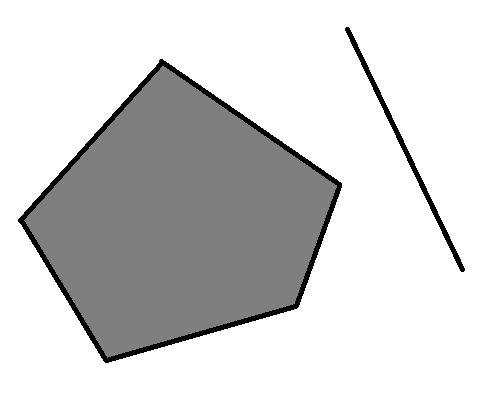
\includegraphics[width=0.4\textwidth ]{ch3-poly-00.png}}
	\subfigure[情形1.2]{
	\label{fig.poly.1.2}
	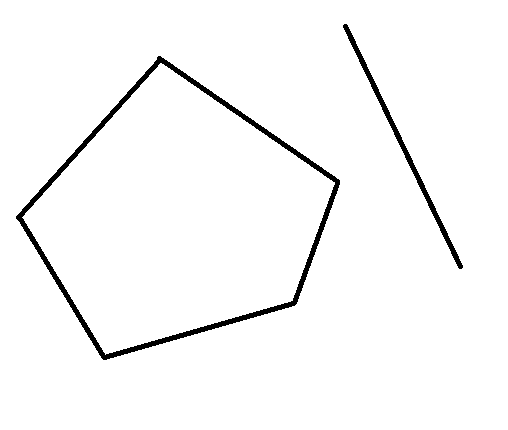
\includegraphics[width=0.4\textwidth ]{ch3-poly-01.png}}
	\caption{直线和多边形位置关系的第一类情形}	 % Caption of figure
	\label{fig.3.beta.l.1}	 % Label of figure
\end{figure}
\item 多边形只有一个顶点和其他顶点不在直线的同一侧,如图\ref{fig.3.beta.l.2}所示又可具体分为两种情况。第一种情况\ref{fig.poly.2.1},只有一个顶点不满足约束,多边形顶点个数加1;第二种情况\ref{fig.poly.2.2},只有一个顶点满足约束,多边形变成一个三角形。
\begin{figure}[htp]
	\centering
	\subfigure[情形2.1]{	 % Caption of subfigure in []
	\label{fig.poly.2.1}	 % Label of subfigure in {}
	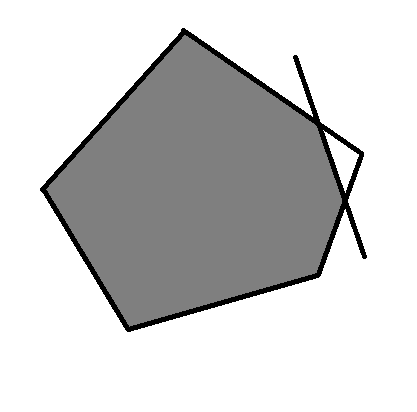
\includegraphics[width=0.4\textwidth ]{ch3-poly-10.png}}
	\subfigure[情形2.2]{
	\label{fig.poly.2.2}
	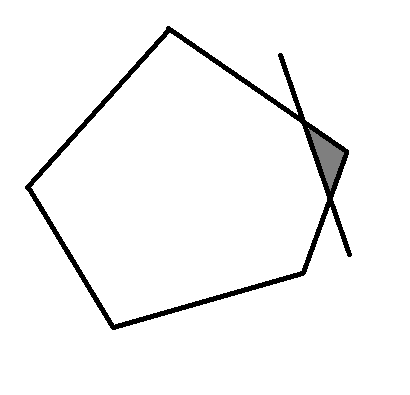
\includegraphics[width=0.4\textwidth ]{ch3-poly-11.png}}
	\caption{直线和多边形位置关系的第二类情形}	 % Caption of figure
	\label{fig.3.beta.l.2}	 % Label of figure
\end{figure}
\item 多边形有至少两个顶点和其他顶点不在直线的同一侧,如图\ref{fig.3.beta.l.2}所示又可具体分为两种情况。图\ref{fig.poly.3.1}和\ref{fig.poly.3.2}是两种对立的情形,事先都无法准确知道剩余的顶点个数,只能根据实际情况确定。
\begin{figure}[htp]
	\centering
	\subfigure[情形3.1]{	 % Caption of subfigure in []
	\label{fig.poly.3.1}	 % Label of subfigure in {}
	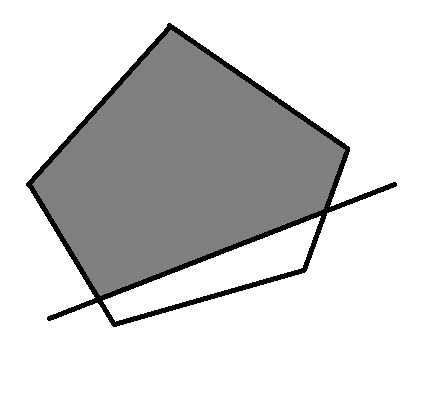
\includegraphics[width=0.4\textwidth ]{ch3-poly-20.png}}
	\subfigure[情形3.2]{
	\label{fig.poly.3.2}
	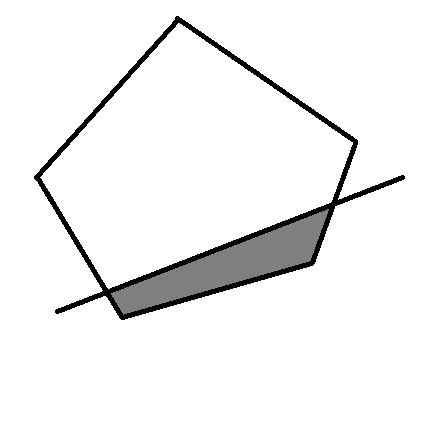
\includegraphics[width=0.4\textwidth ]{ch3-poly-21.png}}
	\caption{直线和多边形位置关系的第三类情形}	 % Caption of figure
	\label{fig.3.beta.l.3}	 % Label of figure
\end{figure}
\end{enumerate}

\section{算法实现}\label{sect:3.3}
\begin{figure}[!h]
 \centering
 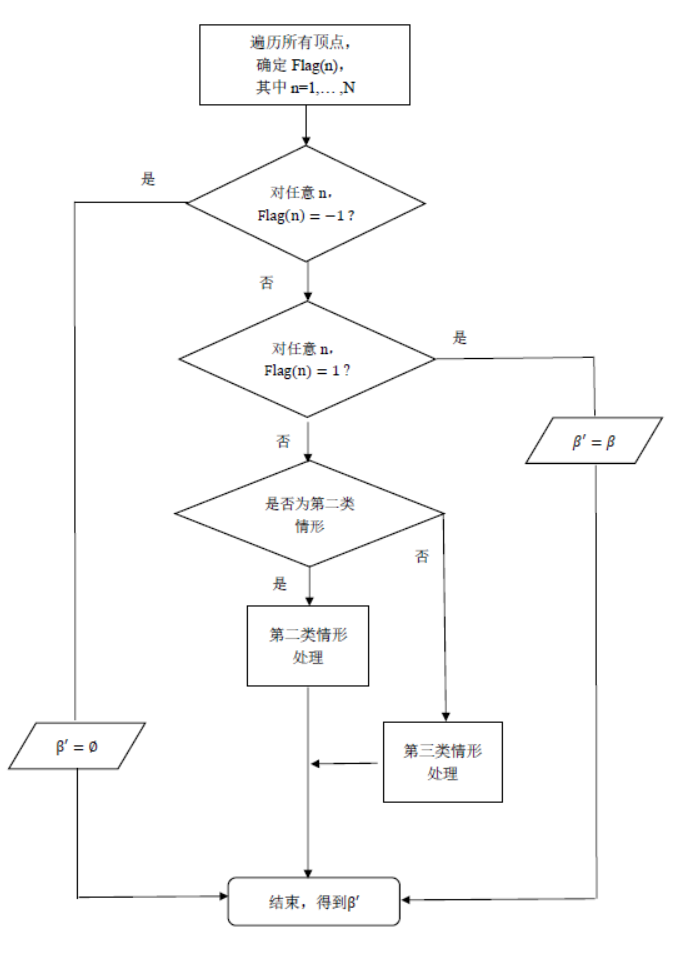
\includegraphics[width=0.9\textwidth ]{ch3-lc-flow.png}\\	 % e.g.,[scale=0.75], [width=0.75\textwidth ]
 \caption{$\mathbf{AddLinear2D}$的算法流程图}
 \label{fig.3.ic.flow}
\end{figure}
根据上节关于多边形和直线的几何位置关系的分析和总结,本节设计了$d_{1}=2$时多边形顶点集变换$\mathbf{AddLinear2D}$的计算几何算法。

需要遍历多边形的所有顶点与多边形的位置关系。可以用一个数组记录顶点$P_{n}$和约束$L_{c}$的位置关系,即
\begin{equation}%
\mathbf{Flag}(n)=\left\{
\begin{array}{ll}
&1\textbf{, for }P_{n}\in L_{c}\\
&-1\textbf{, for }P_{n}\notin L_{c}
\end{array}
\right.
\end{equation}
这里,$n=1,2,\ldots,N$。

根据上节的位置关系结果,设计算法的流程如图\ref{fig.3.ic.flow}所示。最后写出具体过程伪代码实现见算法\ref{alg.ic.2d}。
\begin{algo}%
\caption{$\mathbf{AddLinear2D}$}
\label{alg.ic.2d}
\begin{algorithmic}
\REQUIRE $\Gamma=\{P_{1},P_{2},\ldots,P_{N}\}$\\
\ENSURE $\Gamma'=\{P_{1}',P_{2}',\ldots,P_{N'}'\}$\\
\STATE Denote the number of vertices in $\Gamma$ by $N$
\FOR{$j=1$ to $N$}
	\STATE Denote the $jth$ vertex by $P_{j}$
	\STATE Let $F_{j}=\mathbf{sgn}(c-\phi^{\tau}P_{j})$
\ENDFOR
\IF{$F_{j}\geq0\ \forall 1\leq j\leq n$}
	\STATE $\Gamma'\leftarrow\Gamma$ and return
\ELSIF{$F_{j}<0\ \forall 1\leq j\leq n$}
	\STATE $\Gamma\leftarrow\emptyset$ and return
\ENDIF
\FOR{$j=2$ to $N-1$}
    \IF{($P_{j}$ and $P_{j-1}$ are in different sides) $\bigwedge$ ($P_{j}$ and $P_{j+1}$ are in different sides)}
		\STATE $P_{1}^{i}\leftarrow$ the intersection of $l_{i}$ and $\overline{P_{j-1}P_{j}}$
		\STATE $P_{2}^{i}\leftarrow$ the intersection of $l_{i}$ and $\overline{P_{j+1}P_{j}}$.
		\IF {($F_{j}>0$)}
			\STATE$\Gamma'=\{P_{1}^{i},P_{j},P_{2}^{i}\}$
		\ELSE
			\STATE$\Gamma'=\{P_{1},\ldots,P_{j-1},P_{1}^{i},P_{2}^{i},P_{j+1},\ldots,P_{n}\}$
		\ENDIF
        \STATE break
    \ELSIF{($P_{j},P_{j-1}$ are in different sides) $\bigwedge$ ($P_{j},P_{j+1},\ldots,P_{j+a-1}$ are on the same side) $\bigwedge$ 
		($P_{j+a-1},P_{j+a}$ are on different sides)}
		\STATE $P_{1}^{i}\leftarrow$ the intersection of $l_{i}$ and $\overline{P_{j-1}P_{j}}$
		\STATE $P_{2}^{i}\leftarrow$ the intersection of $l_{i}$ and $\overline{P_{j+a-1}P_{j+a}}$.
		\IF {($F_{j}>0$)}
			\STATE$\Gamma'=\{P_{1}^{i},P_{j},\ldots,P_{j+a-1},P_{2}^{i}\}$
		\ELSE
			\STATE$\Gamma'=\{P_{1},\ldots,P_{j-1},P_{1}^{i},P_{2}^{i},P_{j+a},\ldots,P_{n}\}$
		\ENDIF
        \STATE break
	\ELSIF{($P_{j},P_{j+1}$ are in different sides) $\bigwedge$ ($P_{j},P_{j-1},\ldots,P_{j-b+1}$ are on the same side) $\bigwedge$ 
	($P_{j-b+1},P_{j-b}$ are on different sides)}
		\STATE $P_{1}^{i}\leftarrow$ the intersection of $l_{i}$ and $\overline{P_{j-b+1}P_{j-b}}$
		\STATE $P_{2}^{i}\leftarrow$ the intersection of $l_{i}$ and $\overline{P_{j+1}P_{j}}$.
		\IF {($F_{j}>0$)}
			\STATE$\Gamma'=\{P_{1}^{i},P_{j-b+1},\ldots,P_{j},P_{2}^{i}\}$
		\ELSE
			\STATE$\Gamma'=\{P_{1},\ldots,P_{j-b},P_{1}^{i},P_{2}^{i},P_{j+1},\ldots,P_{n}\}$
		\ENDIF
        \STATE break
    \ENDIF
	\STATE $j\leftarrow j+1$
\ENDFOR
\STATE return $\Gamma'$
\end{algorithmic}
\end{algo}

算法\ref{alg.ic.2d}实现了第\ref{sect:3.1}中提到的信息浓缩估计的第一步。对于第二步,一般选择多边形$\Gamma'$的中心作为参数估计值$\hat{\bm{\theta}}'$,即
\begin{equation}\label{eq.3.theta}
\begin{split}%
&\hat{\theta}_{1}'=\frac1N\sum_{n=1}^{N}X_{P'_{n}}\\
&\hat{\theta}_{2}'=\frac1N\sum_{n=1}^{N}Y_{P'_{n}}
\end{split}
\end{equation}

本节设计的算法\ref{alg.ic.2d}和方程\eqref{eq.3.theta}就是$d_{1}=2$时完整的信息浓缩估计算法,可以用于后续的控制器设计。

\section{仿真实例}\label{sect:3.4}
为了验证本章设计算法的有效性,本节在实际的被控对象中仿真上面设计的信息浓缩估计算法。选择如下的被控对象
\begin{equation}
\label{eq.3.sys.eq}
y_{k+1}=\theta_{1}\cdot y_{k} +\theta_{2}\cdot y_{k-1}+u_{k}+\epsilon_{k+1}+\sin(\frac{k}2)
\end{equation}
其中$\theta_{1}=-0.5$,$\theta_{2}=0.5$。随机干扰取为均匀分布,即
\begin{equation*}
\omega_{k}\in U(0,1) 
\end{equation*}
则随机干扰的上下确界为
\begin{equation*}
0\leq\omega_{k}\leq1
\end{equation*}
而非线性部分是三角函数,其上下界为
\begin{equation*}
-1\leq\sin(\frac{k}2)\leq1
\end{equation*}

为了便于计算,令$u_{k}=0$。在本节中,为了更加符合实际情况,在计算时,将随机干扰和非线性函数的上下界范围扩大,分别取为
\begin{equation*}
-1\leq\omega_{k}\leq2
\end{equation*}
和
\begin{equation*}
-2\leq\sin(\frac{k}2)\leq2
\end{equation*}
因此,合并得到
\begin{equation*}
\underline{z}=-3,\ \overline{z}=4
\end{equation*}
初始的参数集合取为
\begin{equation*}%
\Theta=\{-1\leq\theta_{1}\leq1,\ -1\leq\theta_{2}\leq1\}
\end{equation*}

仿真到第$k=500$时,得到的多边形如图\ref{fig.3.poly}所示,分别以两个参数代表横纵坐标,星形点*代表真实值$\bm{\theta}$在几何坐标轴上的表示,红色圈点代表了估计值$\hat{\bm{\theta}}$在几何坐标轴上的表示。画出整个仿真过程的参数估计曲线如图\ref{fig.3.theta.hat}所示。从这个图中可以看出,参数估计值接近真实值,误差在半径为0.05的球域范围内。
\begin{figure}[!h]
	\centering
	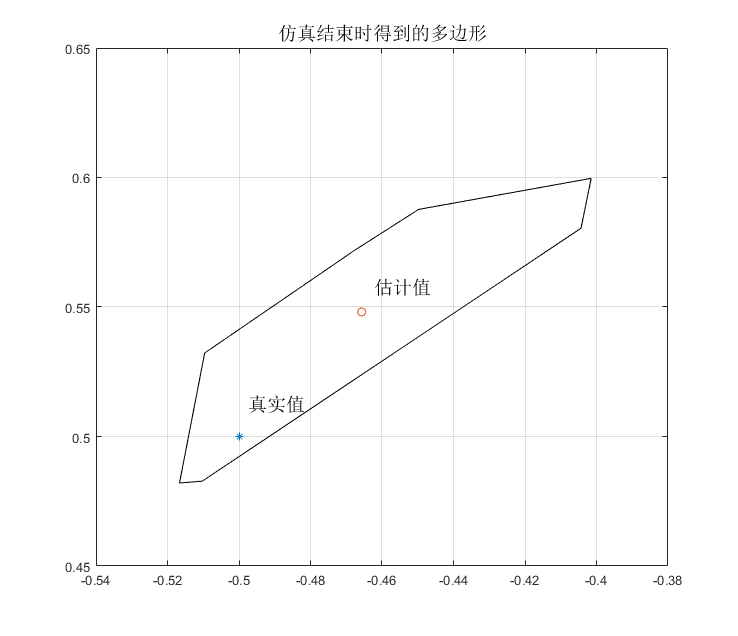
\includegraphics[width=0.7\textwidth ]{ch3-2d-poly.png}\\	 % e.g.,[scale=0.75], [width=0.75\textwidth ]
	\caption{当$d_{1}=2$时仿真实例中$k=500$时的多边形及参数估计}
	\label{fig.3.poly}
\end{figure}

\begin{figure}[!h]
	\centering
	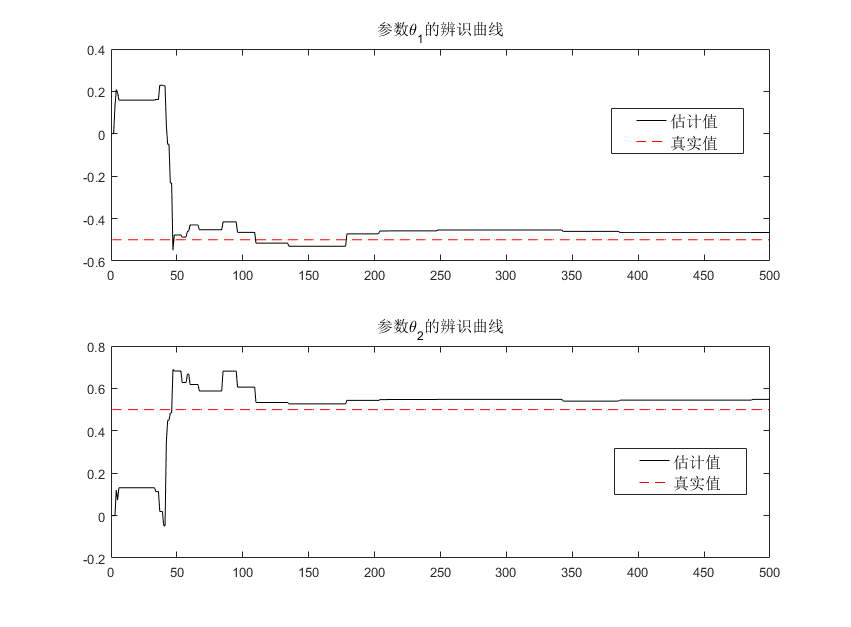
\includegraphics[width=0.8\textwidth ]{ch3-2d-theta.png}\\	 % e.g.,[scale=0.75], [width=0.75\textwidth ]
	\caption{当$d_{1}=2$时仿真实例中的参数估计曲线(信息浓缩估计算法)}
	\label{fig.3.theta.hat}
\end{figure}

\section{优化问题}\label{sect:3.5}
在信息浓缩估计方法中,关键的问题在于计算每一步(时刻$k$)的信息集$I_{k}$和信息浓缩集$C_{k}$。从上面的讨论中,可以看出$d_{1}=1$时很容易解决这两个集合的计算问题。然而,当$d_{1}>1$时,通常情况下集合$C_{k}$中的顶点个数$N_{k}$随着$k\rightarrow\infty$会不断增长,特别是高维情形$d_{1}\geq3$时。因此,有可能在实际应用中,随着$k\rightarrow\infty$,信息浓缩估计过程需要的内存会无限增长,这是一个十分致命的问题,需要优化。

其实,随着$k\rightarrow\infty$,$C_{k}$的范围是在不断缩小的,即使顶点个数可能会增加。因此,为了克服顶点个数无限增长的问题,在实际应用中,可以不需要如此多的顶点来精确的表示信息浓缩集$C_{k}$。也就是说,在多维情形中,在每个时刻$k$的$G$变换过程中,可以用具有足够少顶点个数$N_{L}$的集合$\hat{C}_{k}$来近似$C_{k}$。

一般有两种优化策略,这里主要介绍被称为信息浓缩估计算法的“松实现”(Loose IC estimator, Loose-IC),另外一种是“紧实现”(Tight IC estimator, Tight-IC)。Loose-IC的具体要求是,对于任意的$k$,都满足$\hat{C}_k\supseteq C_k$.

记$$\hat{C}_{\infty}=\bigcap\limits_{k=1}^{\infty} \hat{C}_{k},$$
则
\begin{equation}\label{eq.loose}
C_{\infty}=\bigcap\limits_{k=1}^{\infty} C_{k}\subseteq \hat{C}_{\infty}
\end{equation}

上面的方程\eqref{eq.loose}意味着,Loose-IC在实施过程中不会丢弃任何可能的参数值。对于$d_{1}=2$这种二维情形,为了便于计算,一般选择顶点个数$N_{L}=3$或者$N_{L}=4$,分别如图\ref{fig.3.loose.3}和\ref{fig.3.loose.4}所示。从图中可以看出,顶点个数的减少和多边形的简化,意味者计算复杂度的降低,实现较好的优化效果。

\begin{figure}[!h]
	\centering
	\subfigure[用三角形$Q_{1}Q_{2}P_{4}$近似多边形$P_{1}P_{2}P_{3}P_{4}P_{5}$]{	 % Caption of subfigure in []
	\label{fig.3.loose.3}	 % Label of subfigure in {}
	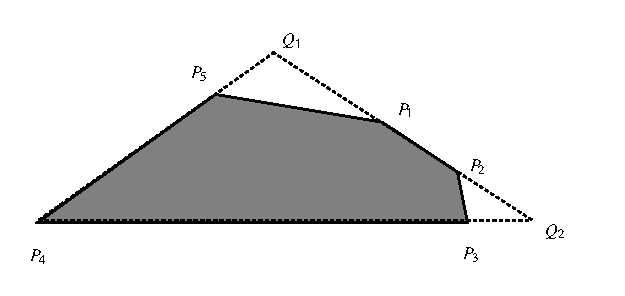
\includegraphics[width=0.7\textwidth ]{ch3-fig-loose-export.eps}}
	\subfigure[用由上下边界围成的矩形近似多边形$P_{1}P_{2}P_{3}P_{4}P_{5}$]{
	\label{fig.3.loose.4}
	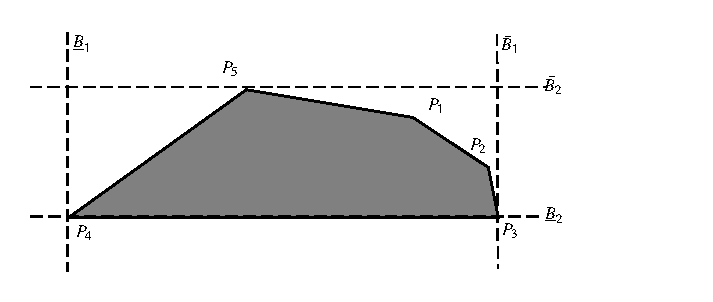
\includegraphics[width=0.7\textwidth ]{ch3-fig-rect-export.eps}}
	\caption{$d_{1}=2$时Loose-IC的实现途径\upcite{}}	 % Caption of figure
	\label{fig.3.loose}	 % Label of figure
\end{figure}

\section{主要特点}\label{sect:3.6}
从上面的讨论和仿真实例中,可以总结出信息浓缩估计算法有如下优点:
\begin{enumerate}
\item 充分利用先验信息和后验数据产生的信息。理想情况下没有任何的信息被浪费掉,而一般传统的辨识算法仅仅利用了部分先验信息和某些随机先验假设。
\item 这是基于集合的估计,实际上每次给出的是一个参数可行的集合,不同于最小二乘算法等给出的点估计,即单个值。这样一方面可以获得比较全面的参数信息,另一方面可以衡量估计值的准确性。
\item 随着时间的增长,逐步找出最优(最有可能的)参数估计值。在参数估计过程中,同时可以用于检查实际采集的数据和系统模型的先验信息的一致性。
\item 可以针对随机系统,也可以处理非统计语言描述的先验信息,不受限于概率模型。
\item 具体实施比较灵活,主要取决于先验信息的具体表现形式,这也给算法的优化带来了极大的提升空间。例如为了降低计算复杂度,可以用上节讨论的“松实现”。
\item 不像传统辨识算法一样,在某些时候表现出随着时间的推移,估计值漂移或者精度下降的现象。相反,数据越多,估计越准确。
\end{enumerate}

一般事物总存在两面性,经过分析,信息浓缩估计算法也存在如下问题:
\begin{enumerate}
\item 难以利用系统干扰项的先验信息,特别是无界随机干扰。也许在这种没有非参数不确定性且随机干扰是无界噪声序列时,传统基于值估计的算法表现得更加适合。
\item 实际的算法效率依赖于先验信息的利用程度和具体实现。一般情况下,由于信息浓缩估计算法涉及到计算几何过程(也许有其他的实施策略),因而其计算复杂度和设计难度要稍大于RLS等传统辨识算法。毕竟后者一般只会涉及到矩阵的加减乘除运算。
\item 目前不存在针对信息浓缩估计算法的显示表达式或者固定的公式,同时,基于集合的辨识思路给具体控制系统的应用和闭环稳定性分析带来了一定的困难。
\end{enumerate}

虽然存在诸如此类的缺点,但信息浓缩估计算法仍然提供了很好的辨识思路和较好的收敛性和精确度,值得深入研究和进一步优化。

\section{本章总结}
本章主要讨论了信息浓缩估计算法的具体实现。首先描述了二维参数情形下,信息浓缩估计算法的主要步骤和基本问题;然后对信息浓缩变换中直线和多边形的几何关系进行了详细地分析,同时设计了信息浓缩变换的算法流程,并给出了具体的伪代码实现;接着在实际的被控对象中仿真本章设计的信息浓缩估计算法,给出了最终估计结果和过程曲线;最后讨论了信息浓缩估计的计算复杂度优化问题,总结了信息浓缩估计的主要优缺点。